\documentclass[10pt,letterpaper, onecolumn]{report}
\usepackage{amsmath}
\usepackage{amssymb}
\usepackage{listings}
\usepackage{xcolor}
\usepackage[lmargin=71pt, tmargin=0.6in]{geometry}
\usepackage{fancyhdr}
\usepackage{graphicx}
\usepackage{subcaption}
\usepackage{enumitem}

% Footer format
\pagestyle{fancy}
\fancyhead{}
\fancyfoot{}
\fancyfoot[L]{Author: Kacper Ragankiewicz, Index: 283415}
\fancyfoot[R]{\thepage}

% Syntax highlighting for Python
\definecolor{keywordcolor}{rgb}{0.58, 0.01, 0.24}
\definecolor{stringcolor}{rgb}{0.44, 0.55, 0.34}
\definecolor{commentcolor}{rgb}{0.5, 0.5, 0.5}
\definecolor{backgroundcolor}{rgb}{0.97, 0.97, 0.97}

\lstdefinestyle{myPythonStyle}{
    language=Python,
    backgroundcolor=\color{backgroundcolor},
    basicstyle=\ttfamily\small,
    keywordstyle=\color{keywordcolor}\bfseries,
    stringstyle=\color{stringcolor},
    commentstyle=\color{commentcolor}\itshape,
    numberstyle=\tiny\color{gray},
    numbersep=5pt,
    stepnumber=1,
    numbers=left,
    showstringspaces=false,
    tabsize=4,
    breaklines=true,
    frame=single,
    rulecolor=\color{black},
}

\renewcommand{\headrulewidth}{0pt}

\begin{document}

% Title
\begingroup
    \centering
    \LARGE \textbf{Complex Systems} \\
    \large CS2024/problem\_6.pdf \\[0.5em]
\endgroup

\begin{flushleft}
    \rule{\textwidth}{0.4pt} \\ % Horizontal line
    \textbf{Result}
\end{flushleft}

\begin{flushleft}
    \begin{flushleft}
        \textbf{Task 1}
        \hfill\break
        \setlength{\parindent}{1.5em} % Adjust paragraph indentation
        \setlength{\parskip}{0.5em}   % Adjust paragraph spacing


        \begin{lstlisting}[style=myPythonStyle, caption={Plot of the lattice LxL}]

import numpy as np
import matplotlib.pyplot as plt
import random
import copy

# Helper function to display lattice
def plot_lattice(lattice, title="Lattice"):
    plt.figure(figsize=(6, 6))
    plt.imshow(lattice, cmap='gray_r', origin='upper')
    plt.title(title)
    plt.colorbar()
    plt.savefig(f"{title}.png")
    plt.show()


def generate_lattice(L, p):
    lattice = np.random.choice([1, 0], size=(L, L), p=[p, 1 - p])
    return lattice

# Parameters
L = 50  # Lattice size
p = 0.4  # Probability of a dog (1)

# Generate and plot lattice
lattice = generate_lattice(L, p)
plot_lattice(lattice, "Initial Lattice")

# Save lattice
np.savetxt("lattice.txt", lattice, fmt='%d')



        \end{lstlisting}

        \begin{figure}[htbp!] % Positioning options: here, top, bottom, page
            \centering
            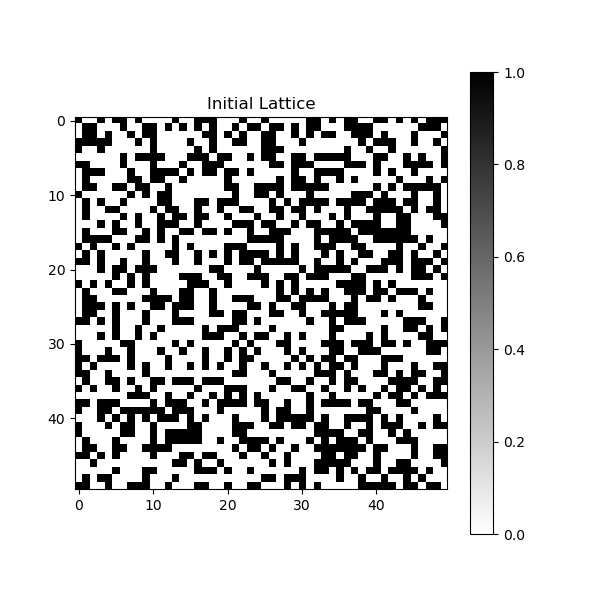
\includegraphics[width=0.29\textwidth]{../Initial Lattice.png} % Specify image file and scale
        \end{figure}

    \end{flushleft}

\end{flushleft}

\clearpage
\begin{flushleft}
    \begin{flushleft}
        \textbf{Task 2}
        \hfill\break
        \setlength{\parindent}{1.5em} % Adjust paragraph indentation
        \setlength{\parskip}{0.5em}   % Adjust paragraph spacing


        \begin{lstlisting}[style=myPythonStyle, caption={Flea on the very left dog}]
import numpy as np
import matplotlib.pyplot as plt
import random
import copy

# Helper function to generate a lattice


def generate_lattice(L, p, immunization_rate=0.0):
    # Generate lattice with dogs (1) and empty spaces (0)
    lattice = np.random.choice([1, 0], size=(L, L), p=[p, 1 - p])

    # Apply immunization by changing a fraction of dogs to immune (3)
    total_dogs = np.sum(lattice == 1)
    num_immunized = int(immunization_rate * total_dogs)
    immunized_positions = random.sample(
        list(zip(*np.where(lattice == 1))), num_immunized)

    for pos in immunized_positions:
        lattice[pos] = 3  # Mark as immunized (3)

    return lattice

# Function to find the first dog in the first row or subsequent rows


def find_first_dog(lattice):
    # Iterate over rows in case the first row is empty
    for i in range(lattice.shape[0]):
        for j in range(lattice.shape[1]):
            if lattice[i, j] == 1:  # Found an infected dog
                return (i, j)
    return None

# Flea simulation with infection spread, including immunization


def simulate_flea_updated(lattice, t):
    # Make a copy to avoid modifying the original
    lattice = copy.deepcopy(lattice)
    flea_pos = find_first_dog(lattice)

    if flea_pos is None:
        print("No dog found in the lattice.")
        return lattice

    x, y = flea_pos
    lattice[x, y] = 2  # Mark the initial position as infected

    for _ in range(t):
        neighbors = [(x-1, y), (x+1, y), (x, y-1), (x, y+1)]
        valid_moves = [(nx, ny) for nx, ny in neighbors if 0 <= nx < lattice.shape[0]
                        and 0 <= ny < lattice.shape[1] and lattice[nx, ny] == 1]

        # Ensure the flea does not infect immunized dogs (marked as 3)
        valid_moves = [
            pos for pos in valid_moves if lattice[pos[0], pos[1]] != 3]

        if not valid_moves:  # If no valid moves, stop the simulation early
            break

        x, y = random.choice(valid_moves)
        lattice[x, y] = 2  # Mark as infected

    return lattice

# Function to calculate epidemic fraction


def updated_epidemic_fraction(lattice, t, num_runs, immunization_rate):
    fractions = []
    for _ in range(num_runs):
        # Generate a new lattice with given immunization rate for each run
        lattice_with_immunization = generate_lattice(
            lattice.shape[0], 0.7, immunization_rate)  # Adjust p and immunization
        infected_lattice = simulate_flea_updated(lattice_with_immunization, t)
        denom = np.sum(infected_lattice > 0)
        fraction = np.sum(infected_lattice == 2) / denom if denom > 0 else 0
        fractions.append(fraction)
    return fractions

# Visualization helper function


def plot_lattice(lattice, title="Lattice"):
    plt.figure(figsize=(6, 6))
    plt.imshow(lattice, cmap='viridis', origin='upper')
    plt.title(title)
    plt.colorbar(label="Cell State")
    plt.show()


# Parameters
L_large = 100  # Larger lattice size
p_high = 0.7  # Higher probability of dogs
t_long = 1000  # Longer simulation time
num_runs = 50  # Number of simulation runs
# Testing different levels of immunization
immunization_rates = [0.1, 0.3, 0.5]

# Run the epidemic fraction analysis for different immunization rates
all_fractions = {}

for immunization_rate in immunization_rates:
    fractions_improved = updated_epidemic_fraction(generate_lattice(
        L_large, p_high), t_long, num_runs, immunization_rate)
    all_fractions[immunization_rate] = fractions_improved

# Plot the updated epidemic size analysis
plt.figure(figsize=(8, 5))
for immunization_rate, fractions in all_fractions.items():
    plt.plot(range(num_runs), fractions, marker='o', linestyle='-',
                label=f'Immunization Rate {immunization_rate}')

plt.xlabel("Simulation Run")
plt.ylabel("Fraction of Infected Nodes")
plt.title("Epidemic Size Over Time (With Immunization)")
plt.legend()
plt.savefig("epidemic_size_with_immunization.png")
plt.show()

# Parameters for flea simulation
t = 100  # Number of jumps

# Create a lattice and run flea simulation
lattice = generate_lattice(L_large, p_high)
infected_lattice = simulate_flea_updated(lattice, t)
plot_lattice(infected_lattice, "Lattice After Flea Movements")

# Save infected lattice to file
np.savetxt("infected_lattice.txt", infected_lattice, fmt='%d')
                    \end{lstlisting}

\begin{figure}[htbp!]
    \centering
    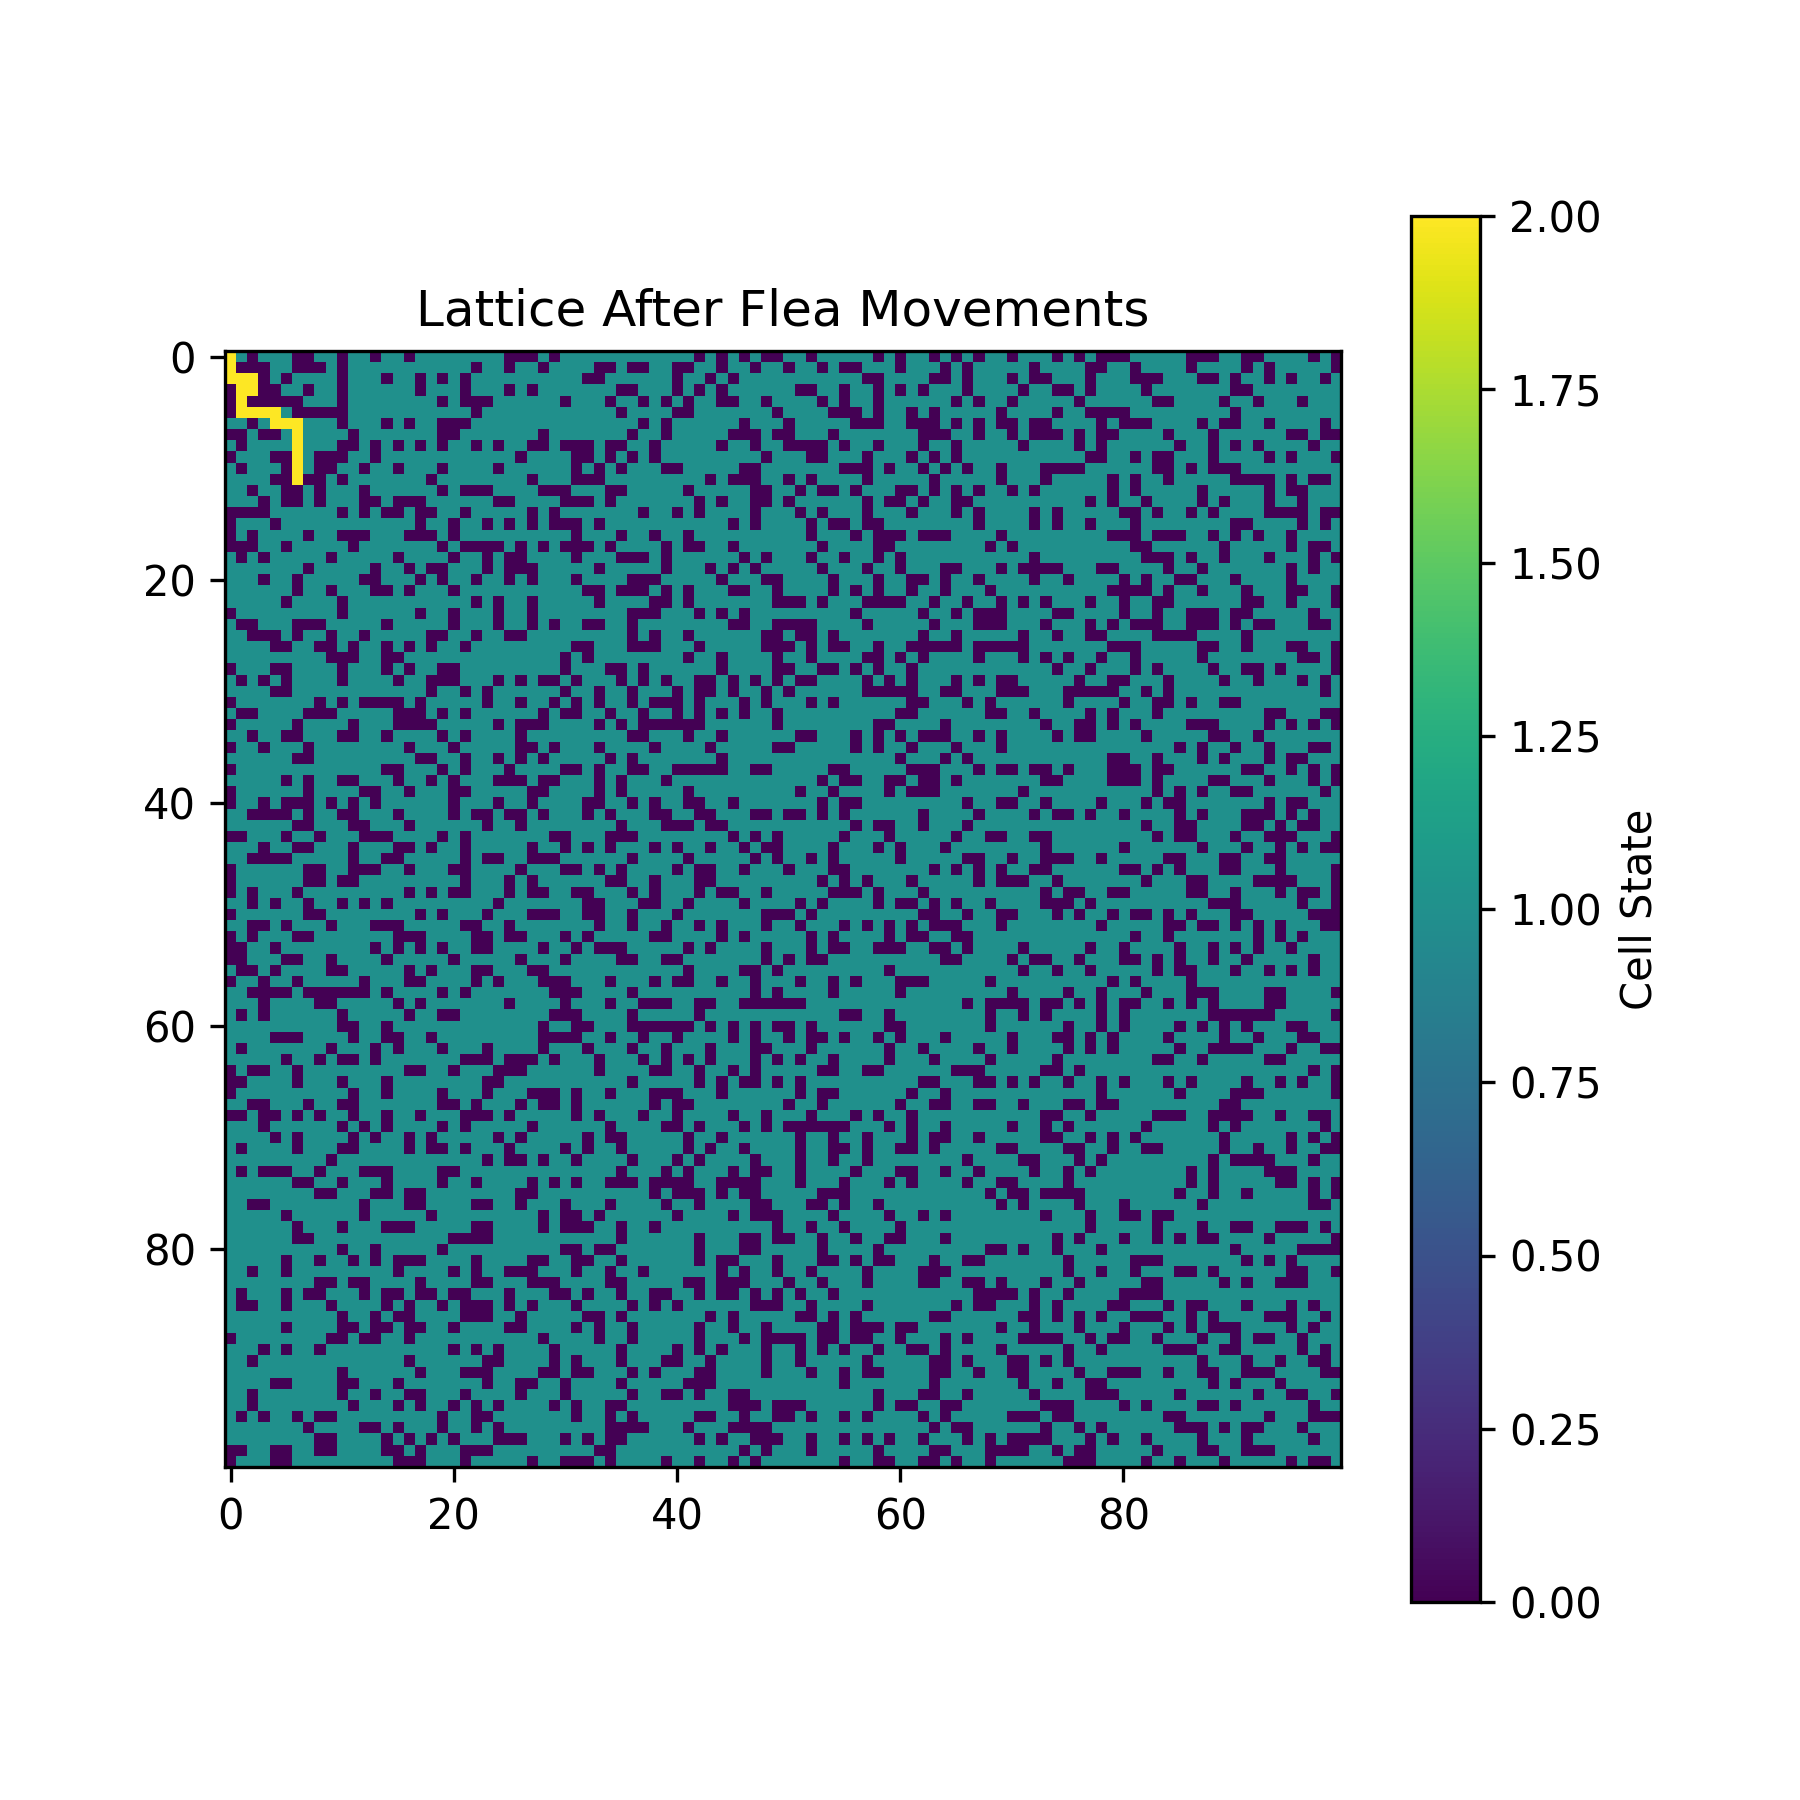
\includegraphics[width=0.7\textwidth]{../Lattice After Flea Movements.png}
    \caption{Lattice After Flea Movements}
\end{figure}

\begin{figure}[htbp!]
    \centering
    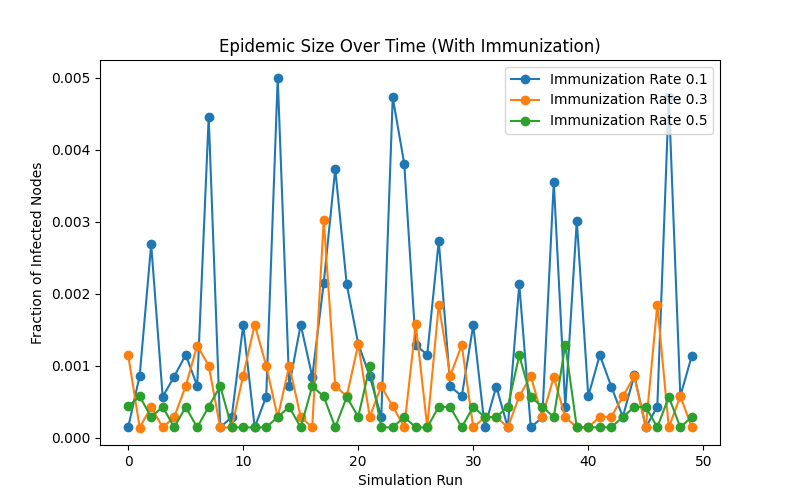
\includegraphics[width=0.7\textwidth]{../epidemic_size_with_immunization.png}
    \caption{Epidemic Size with Immunization}
\end{figure}

    \end{flushleft}

\end{flushleft}

\break\hfill

\begin{flushleft}
    \begin{flushleft}
        \textbf{Task 3}
        \hfill\break
        \setlength{\parindent}{1.5em} % Adjust paragraph indentation
        \setlength{\parskip}{0.5em}   % Adjust paragraph spacing

        Wolfram Cellular Automata

        \begin{lstlisting}[style=myPythonStyle, caption={Flea on the very left dog}]

def wolfram_ca(rule, steps, size):
rule_bin = np.array([int(x) for x in np.binary_repr(rule, width=8)])
ca = np.zeros((steps, size), dtype=int)
ca[0, size // 2] = 1  # Single seed

for i in range(1, steps):
    for j in range(size):
        left = ca[i-1, (j-1) % size]
        center = ca[i-1, j]
        right = ca[i-1, (j+1) % size]
        idx = 7 - (left * 4 + center * 2 + right)
        ca[i, j] = rule_bin[idx]

return ca

# Parameters
steps, size = 50, 100
rules = [18, 26, 181]

plt.figure(figsize=(15, 5))
for i, rule in enumerate(rules):
ca = wolfram_ca(rule, steps, size)
plt.subplot(1, len(rules), i+1)
plt.imshow(ca, cmap='gray', aspect='auto')
plt.title(f"Rule {rule}")

plt.savefig('ca_wolfram.png')
plt.show()
        
        \end{lstlisting}

        \begin{figure}[htbp!] % Positioning options: here, top, bottom, page
            \centering
            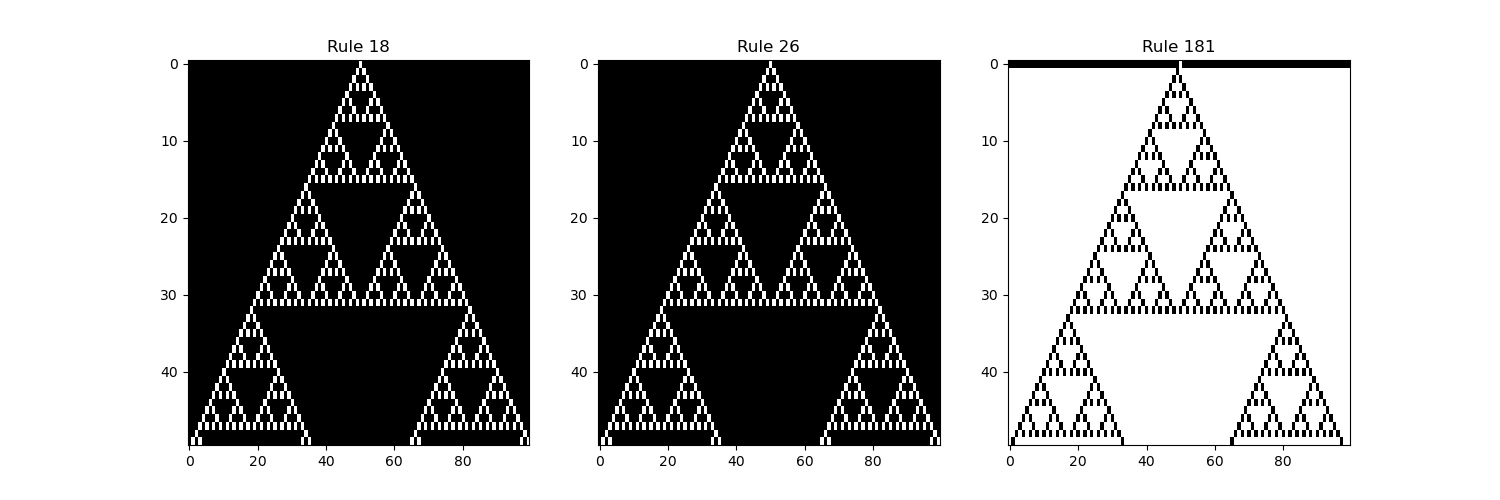
\includegraphics[width=1\textwidth]{../ca_wolfram.png} % Specify image file and scale
        \end{figure}

    \end{flushleft}

\end{flushleft}

\begin{flushleft}
    \begin{flushleft}
        \textbf{Task 5}
        \hfill\break
        \setlength{\parindent}{1.5em} % Adjust paragraph indentation
        \setlength{\parskip}{0.5em}   % Adjust paragraph spacing


        \begin{lstlisting}[style=myPythonStyle, caption={Game of Life}]
from scipy.signal import convolve2d
import numpy as np
import matplotlib.pyplot as plt

# Game of Life step function


def game_of_life_step(grid):
    kernel = np.array([[1, 1, 1], [1, 0, 1], [1, 1, 1]])
    neighbors = convolve2d(grid, kernel, mode='same', boundary='wrap')
    return ((neighbors == 3) | ((grid == 1) & (neighbors == 2))).astype(int)

# Plot lattice helper function


def plot_lattice(grid, title="Grid"):
    plt.figure(figsize=(6, 6))
    plt.imshow(grid, cmap="gray_r", origin="upper")
    plt.title(title)
    plt.colorbar(label="Cell State")
    plt.show()


# Initialize grid with a glider pattern
L = 50
grid = np.zeros((L, L), dtype=int)

# Add a glider pattern
glider = np.array([[0, 1, 0],
                    [0, 0, 1],
                    [1, 1, 1]])

# Place the glider in the grid
grid[1:4, 1:4] = glider

# Run simulation
for step in range(10):
    plot_lattice(grid, f"Game of Life - Step {step}")
    grid = game_of_life_step(grid)
                    
                    \end{lstlisting}

                    \begin{figure}[htbp!] % Positioning options: here, top, bottom, page
                        \centering
                        \begin{minipage}{0.3\textwidth}
                            \centering
                            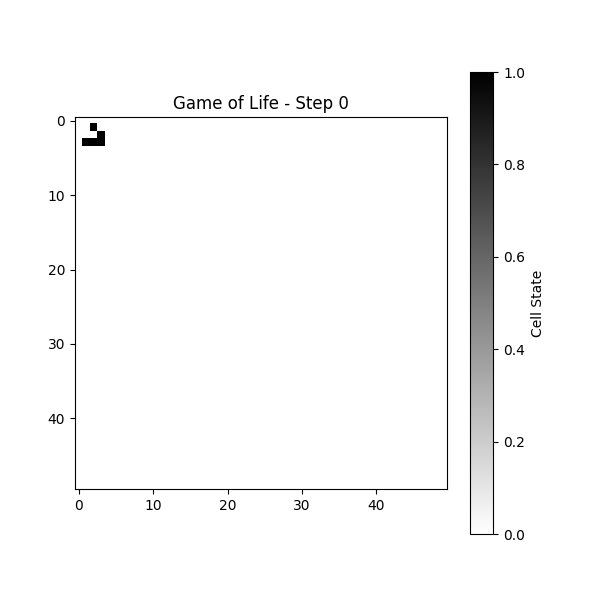
\includegraphics[width=\textwidth]{../game_of_life_step_Game of Life - Step 0}
                            \caption{Step 0}
                        \end{minipage}%
                        \begin{minipage}{0.3\textwidth}
                            \centering
                            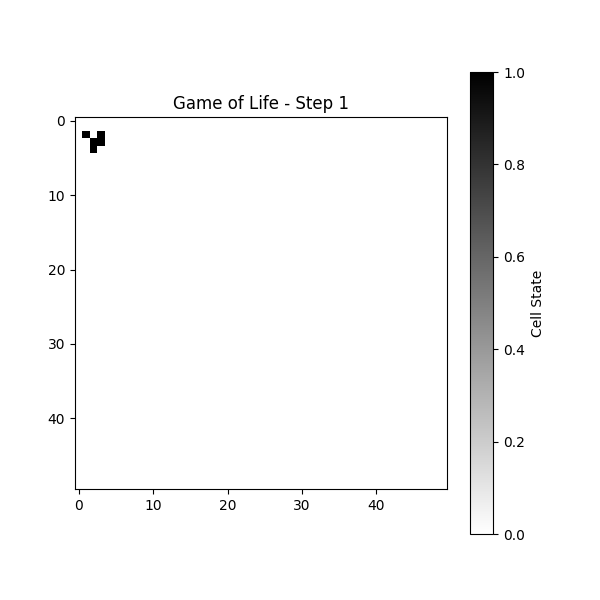
\includegraphics[width=\textwidth]{../game_of_life_step_Game of Life - Step 1}
                            \caption{Step 1}
                        \end{minipage}%
                        \begin{minipage}{0.3\textwidth}
                            \centering
                            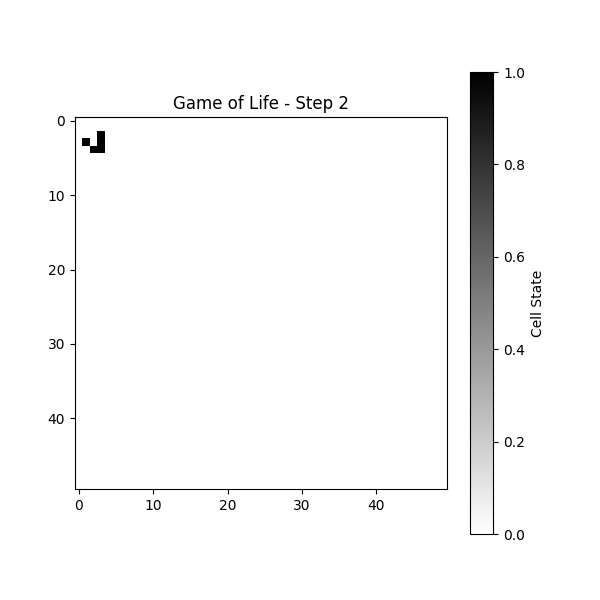
\includegraphics[width=\textwidth]{../game_of_life_step_Game of Life - Step 2}
                            \caption{Step 2}
                        \end{minipage}
                        \vspace{0.5cm} % Adds vertical space between rows
                    
                        \begin{minipage}{0.3\textwidth}
                            \centering
                            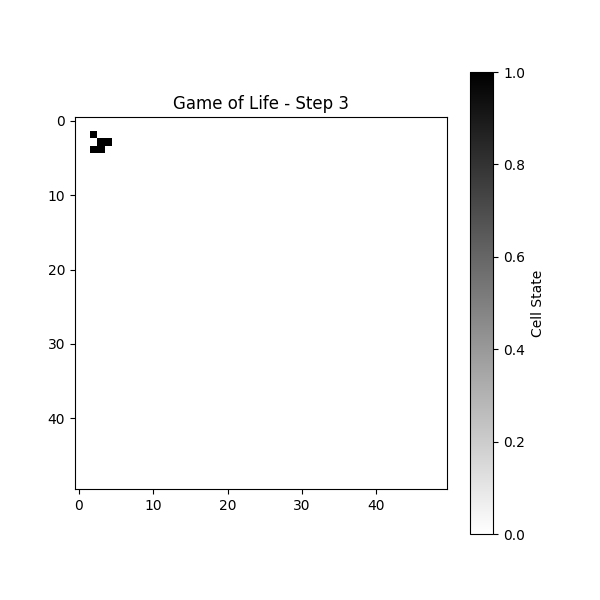
\includegraphics[width=\textwidth]{../game_of_life_step_Game of Life - Step 3}
                            \caption{Step 3}
                        \end{minipage}%
                        \begin{minipage}{0.3\textwidth}
                            \centering
                            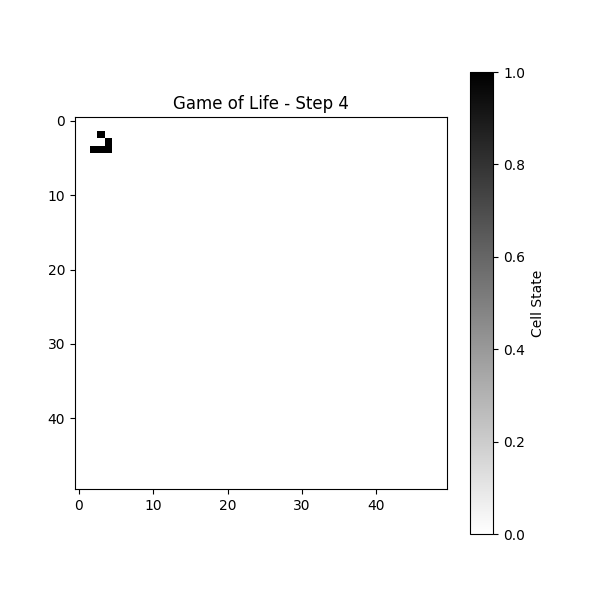
\includegraphics[width=\textwidth]{../game_of_life_step_Game of Life - Step 4}
                            \caption{Step 4}
                        \end{minipage}%
                        \begin{minipage}{0.3\textwidth}
                            \centering
                            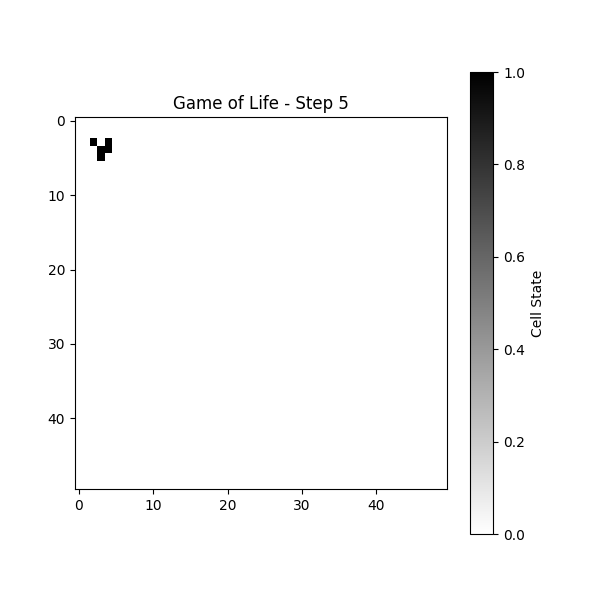
\includegraphics[width=\textwidth]{../game_of_life_step_Game of Life - Step 5}
                            \caption{Step 5}
                        \end{minipage}
                        \vspace{0.5cm} % Adds vertical space between rows
                    
                        \begin{minipage}{0.3\textwidth}
                            \centering
                            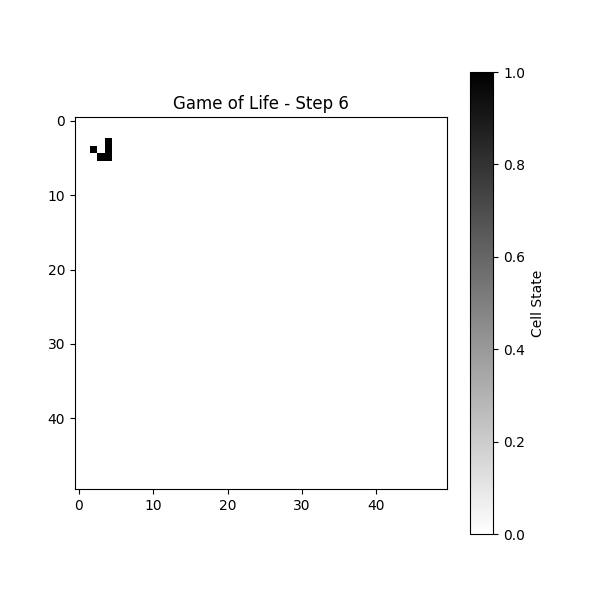
\includegraphics[width=\textwidth]{../game_of_life_step_Game of Life - Step 6}
                            \caption{Step 6}
                        \end{minipage}%
                        \begin{minipage}{0.3\textwidth}
                            \centering
                            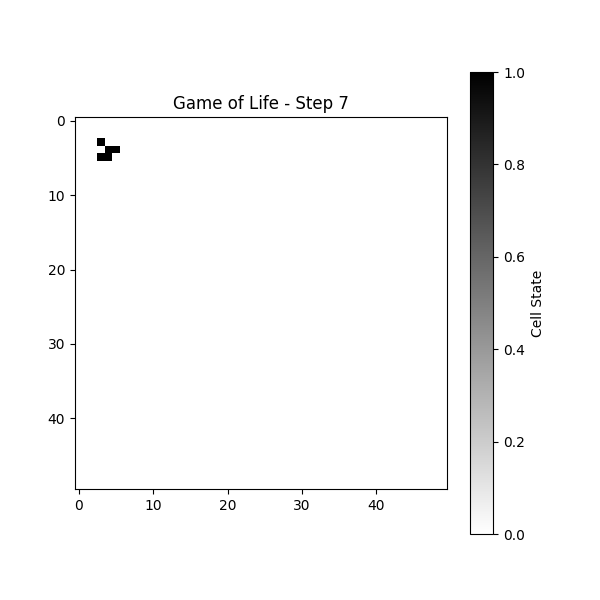
\includegraphics[width=\textwidth]{../game_of_life_step_Game of Life - Step 7}
                            \caption{Step 7}
                        \end{minipage}%
                        \begin{minipage}{0.3\textwidth}
                            \centering
                            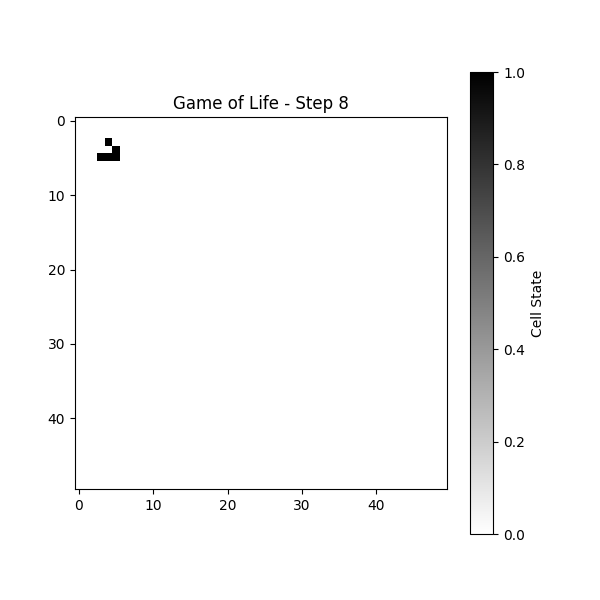
\includegraphics[width=\textwidth]{../game_of_life_step_Game of Life - Step 8}
                            \caption{Step 8}
                        \end{minipage}
                        \caption{Game of Life Steps from 0 to 8}
                    \end{figure}
                    

    \end{flushleft}

\end{flushleft}



\end{document}
